\documentclass[main.tex]{subfiles} % Subfile-Class



% ============================================================================== %
%                            Subfile document                                    %
% ============================================================================== %

\begin{document}

% Template

\subsubsection{Liniensensor}

Im folgenden Abschnitt ist die Entwicklung und Evaluierung eines Liniensensors
dokumentiert. Ziel ist es, einen einfach auszuwertenden Sensor zu entwickeln,
der das vorgegebene Klebeband (\textit{Tesa Gewebeband 4651}) problemlos vom Wettkampf-Untergrund unterscheiden kann.\\
Ein eigener Liniensensor wird entwickelt, weil das Verlassen der Strecke als ein hohes Risiko empfunden wird. Daher ermöglicht
das eigene Designen eines Liniensensors eine hohe flexibilität. Dies mit der Begründung, dass für ein massgeschneidertes Produkt 
die optimalen Komponenten selber erlesen werden können und weil man mit dem selbst gebauten Produkt bestens vertraut ist.


% ===================================================================================
\paragraph{Anforderungen}

Das Klebeband muss auf einem rötlich
gefliesten Untergrund detektiert werden. Eine besondere Herausforderung
stellen hierbei längs und querverlaufende Fliesenfugen dar, welche eine
ähnliche Farbe aufweisen. Dieser Untergrund ist in
Abbildung~\ref{fig:Untergrund_Wettkampf} gezeigt.

\begin{figure}[H]
    \centering
    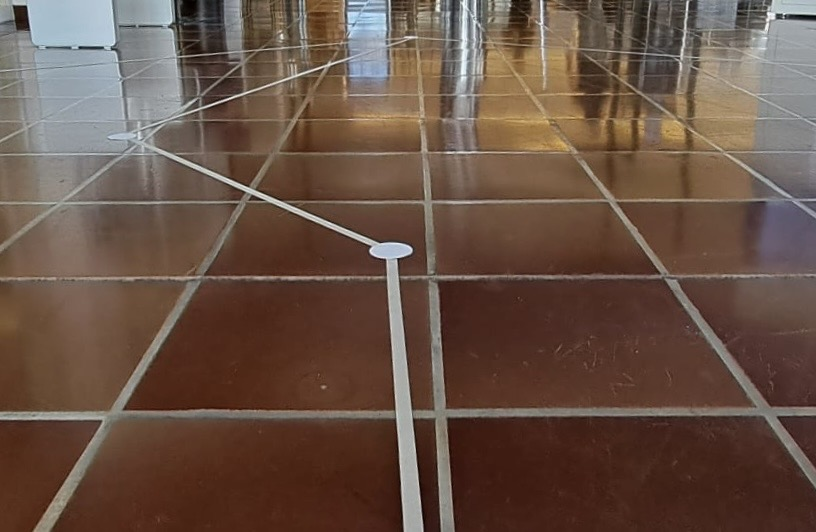
\includegraphics[width=0.75\textwidth]{fig_Strecke_Tracken/Bild_Untergrund.jpg}
    \caption{Untergrund während des Wettkampfs}~\label{fig:Untergrund_Wettkampf}
\end{figure}

% ===================================================================================
\paragraph{Konzeptionierung}

\subsubsection{Aufbau und Auswertung}
Der Liniensensor wird aus acht einzelnen Messzellen aufgebaut. Es werden acht Messzellen
gewählt, damit eine möglichst breite Fläche durch den Sensor abgedeckt werden kann, aber
dennoch nicht zu viele Pins für die Auswertung benötigt werden. Dabei sollten stets genau
zwei Messzellen direkt über dem Klebeband ausgerichtet sein. Jede einzelne Messzelle hat 
eine emittierende Diode und einen dazugehörigen Fototransistor. Je mehr Licht auf den 
Fototransistor einwirkt, desto höher ist der Strom, welcher durch ihn fliesst. Weil der 
Fototransistor als konstante Stromquelle interpretiert werden kann, wird der Spannungsabfall
über ihn ausgewertet. Ein hoher Strom durch den Fototransistor bewirkt einen hohen 
Spannungsverlust an einem davor geschaltenen Widerstand. Somit sollte die Spannung über dem
Fototransistor gegen Ground gezogen werden. Ist der Strom jedoch klein,
so fällt gemäss dem Ohmschen Gesetz wenig Spannung über dem Vorwiderstand ab was einen erhöhten
Spannungsabfall über dem Fototransistor zur Folge hat. Diese Spannungen werden dann mittels
Analog-Digital-Wandlern (ADC) ausgewertet. In Abbildung~\ref{fig:Auswertung_Liniensensor1} ist 
die Auswertung bildlich festgehalten.

\begin{figure}[H]
    \centering
    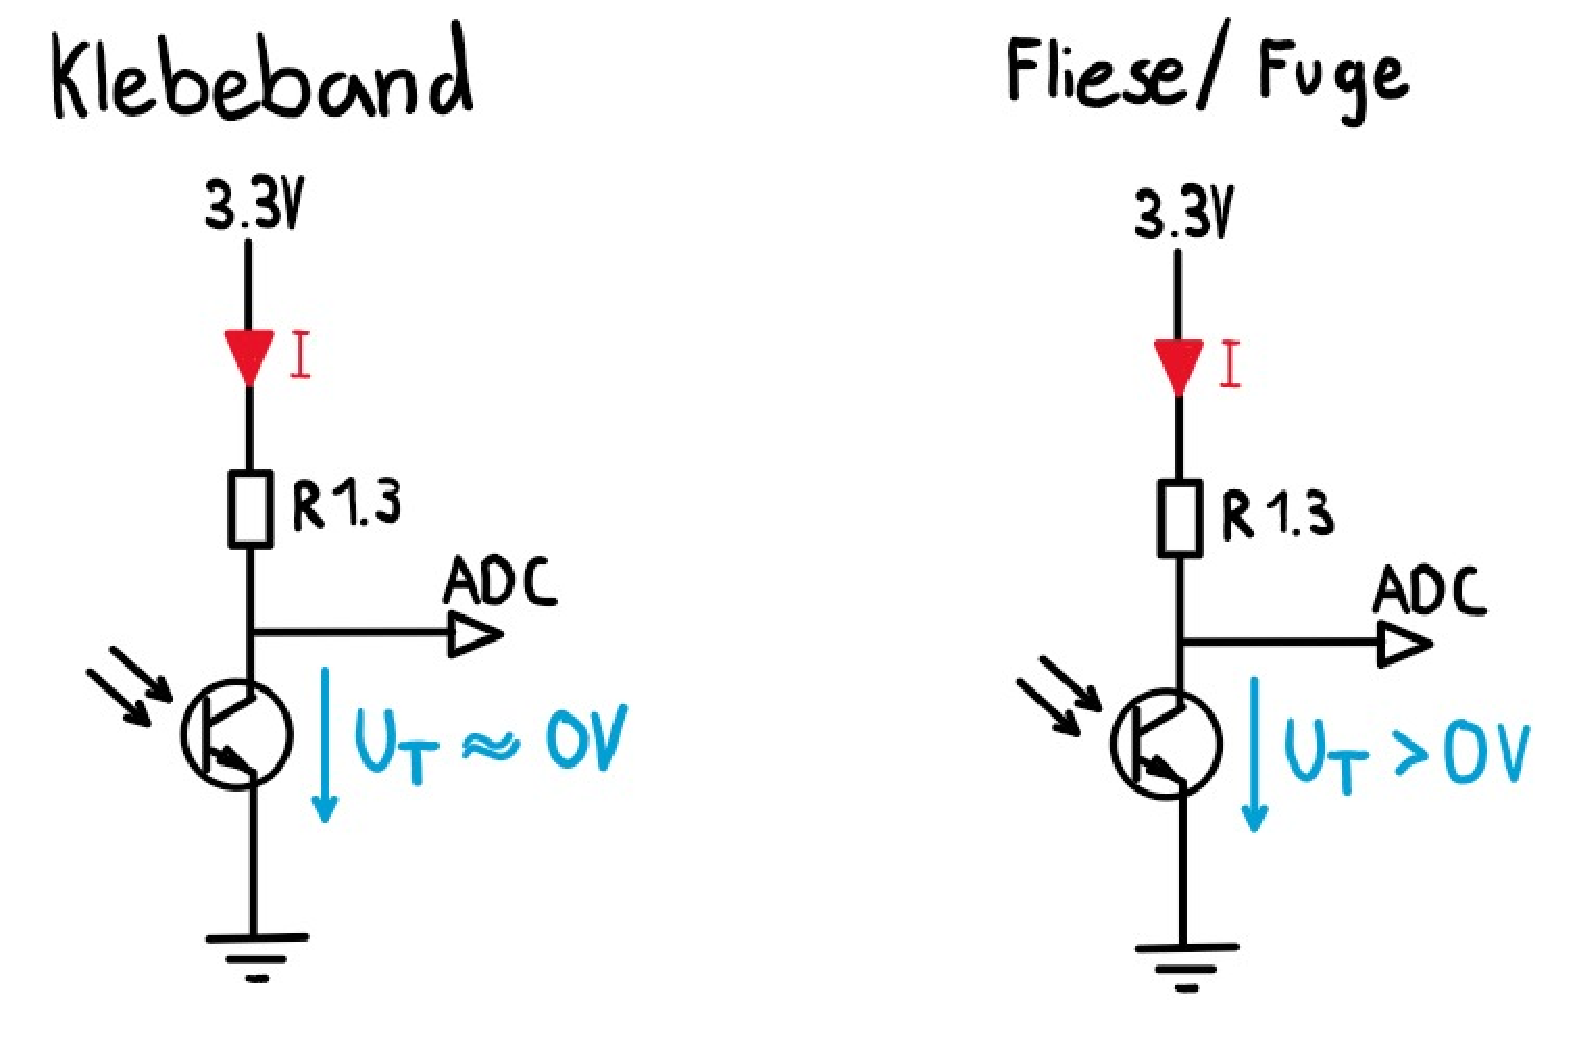
\includegraphics[width=0.5\textwidth]{fig_Strecke_Tracken/Auswertung_Liniensensor.pdf}
    \caption{Konzept der Auswertung mittels ADC}~\label{fig:Auswertung_Liniensensor1}
\end{figure}

% ======================================================================================
\subsubsection{Wahl des Lichtspektrums}
Damit der Unterschied zwischen dem Wettkampfuntergrund und dem Klebeband möglichst 
drastisch hervorgehoben werden kann, ist zuerst eine Evaluierung des optimalen
Lichtspektrums nötig. Im Anhang~\ref{anhang:Liniensensor_Lichtspektrum} sind Versuche dokumentiert, welche die Spannungen 
über dem Fototransistor im Infrarot-Spektrum (IR) und im Ultraviolett-Spektrum (UV) 
dokumentiert. Dabei wird für ersteres ein Emitter und ein Fototransistor im IR-Spektrum (beide 940 nm Peak-Wellenlänge)
verwendet. Beim Versuch im UV-Spektrum wird ein UV-Emitter (395nm Peak-Wellenglänge) mit einem Fototransistor (630nm Peak-Wellenlänge) 
im sichtbaren Spektrum verwendet. Dabei wird eine fluoreszierende Wirkung des Klebebandes 
vermutet. Gemäss der Dokumentation im Anhang ist in der Tat eine fluoreszierende Wirkung des Klebebandes 
ersichtlich. Aufgrund der deutlicheren Ergebnissen im UV-Spektrum als im IR-Spektrum wird auf einen 
UV-Emitter mit einem Fototransistor im sichtbaren Lichtspektrum zurückgegriffen.


% ===================================================================================
\subsubsection{Geometrische Überlegungen}
Abbildung~\ref{fig:Konzept_graphml} zeigt die konzeptionellen Überlegungen einer Messzelle des
Liniensensors. Gemäss dem Datenblatt hat der UV-Emitter (Sender) einen Abstrahlwinkel von 15° und der
Fototransistor (Empfänger) einen Einfallswinkel von 60°. Für eine möglichst störungsfreie Detektion muss auf dem Boden 
eine möglichst grosse Fläche des Empfänger-Kreises durch den Sender-Kreis ausgefüllt werden.\\
Diese einzelnen Messzellen sollen untereinander und von der Umwelt abgekapselt werden. Dies
mit der Begründung, dass die Fototransistoren, gegebenenfalls empfindlich auf
Umwelteinflüsse reagieren könnten. Daher wird ein Gehäuse für die Abschirmung von Umwelteinflüssen
notwendig.

\begin{figure}[H]
    \centering
    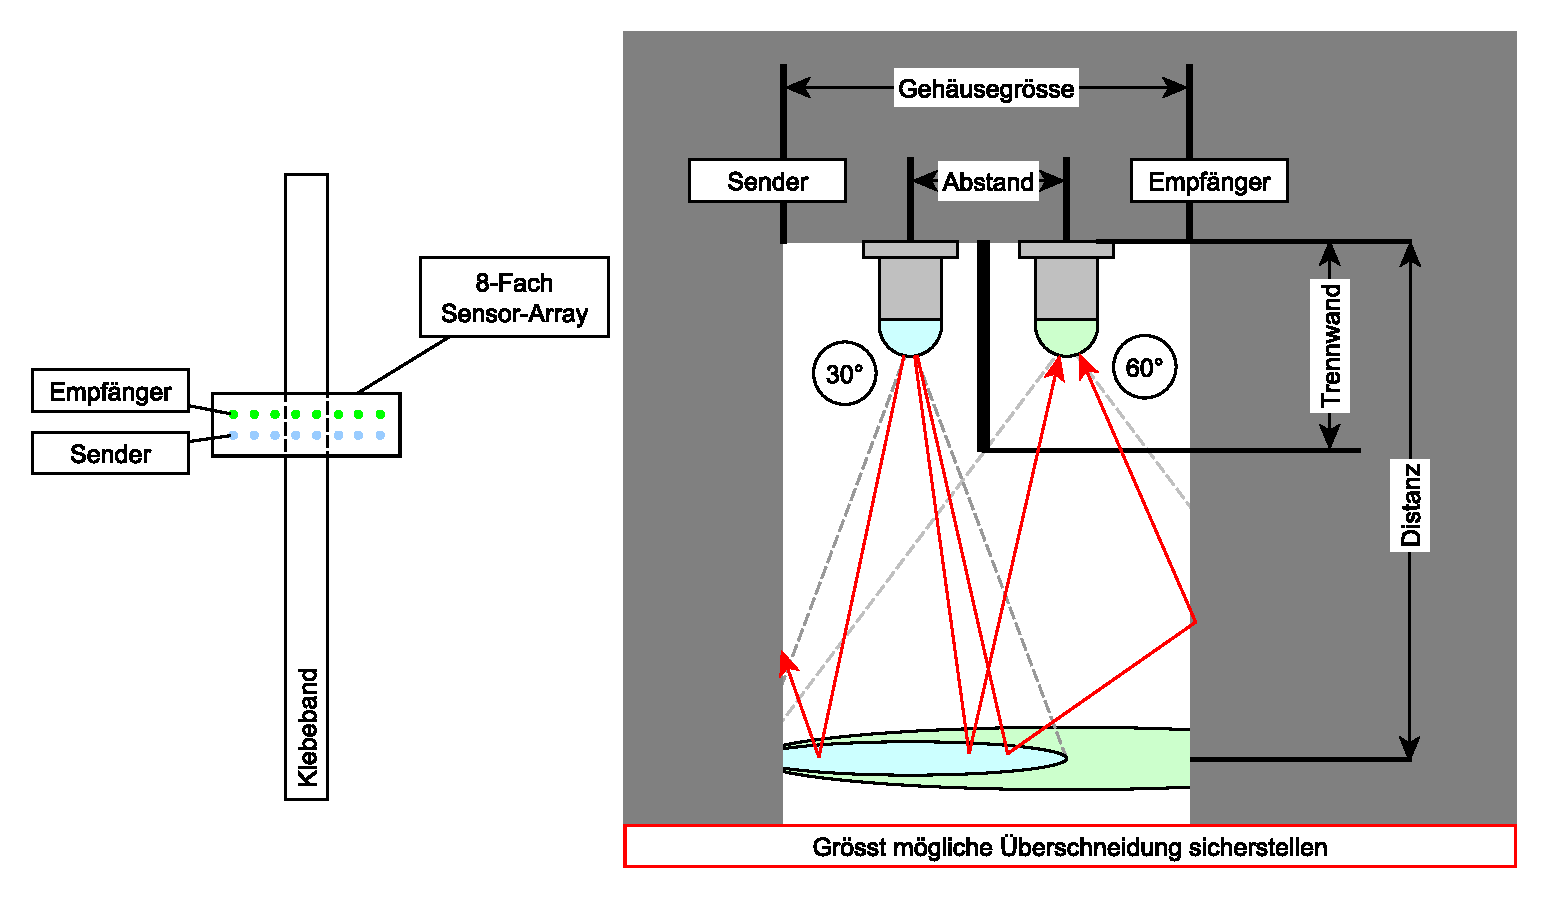
\includegraphics[width=0.75\textwidth]{fig_Strecke_Tracken/Konzept.pdf}
    \caption{Konzept des Liniensensors}~\label{fig:Konzept_graphml}
\end{figure}


% ===================================================================================

\subsubsection{Dimensionierung Gehäuse}
Damit der Empfänger möglichst wenig auf Umwelteinflüsse reagiert, wird nun ein 
Gehäuse dimensioniert, welches den Sensor abschirmen soll. Die nachfolgende 
Abbildung~\ref{fig:Gehaeuse_Vermasst} zeigt eine Skizze, welche den Aufbau des Gehäuses repräsentiert.
In dieser Skizze wird jeder Emitter und Fototransistor von allen anderen abgeschottet. Die vier Löcher
passen genau auf das PCB des Liniensensors. Die Höhe des Gehäuses, stellt den Abstand zwischen Liniensensor
und dem Boden dar. Der grösste Stromdifferenz wurde in einer Höhe von 2.5 cm gemessen. Daher wurde die Höhe
des Gehäuses auf 2.5 cm festgelegt.
Die isometrische Ansicht des Gehäuse ist in Abbildung~\ref{fig:Gehaeuse_Isometrisch} !!!!!Anpassen!!!!!!



\begin{figure}[H]
    \centering
    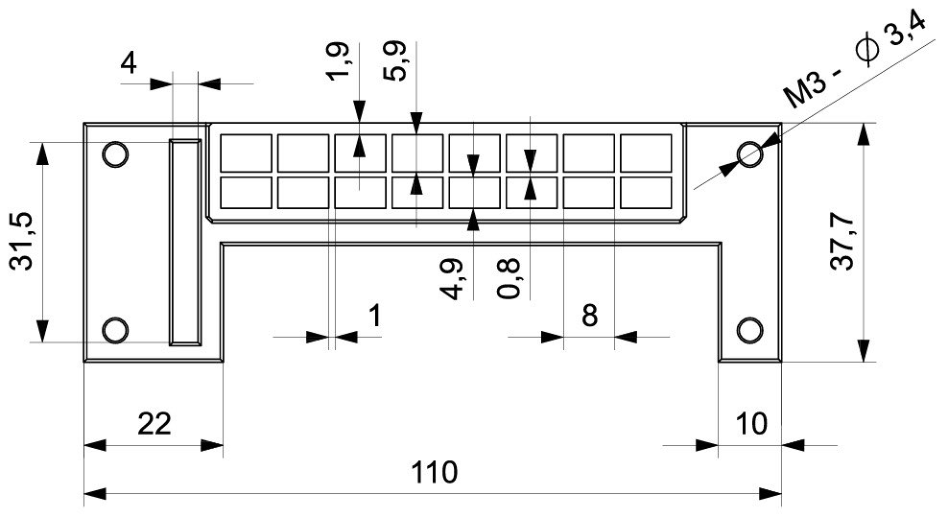
\includegraphics[width=0.75\textwidth]{fig_Strecke_Tracken/Gehaeuse_Vermasst.pdf}
    \caption{Vermassung des Gehäuses in Siemens NX}~\label{fig:Gehaeuse_Vermasst}
\end{figure}

\begin{figure}[H]
    \centering
    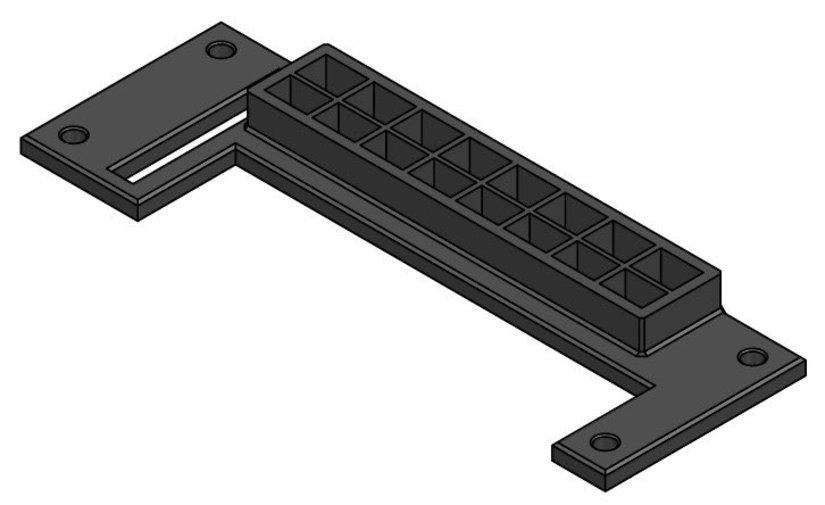
\includegraphics[width=0.75\textwidth]{fig_Strecke_Tracken/Gehaeuse_Isometrisch.pdf}
    \caption{Isometrische Ansicht des Gehäuses in Siemens NX}~\label{fig:Gehaeuse_Isometrisch}
\end{figure}



% ===================================================================================

\subsubsection{Elektrotechnische Dimensionierung}

\begin{figure}[H]
    \centering
    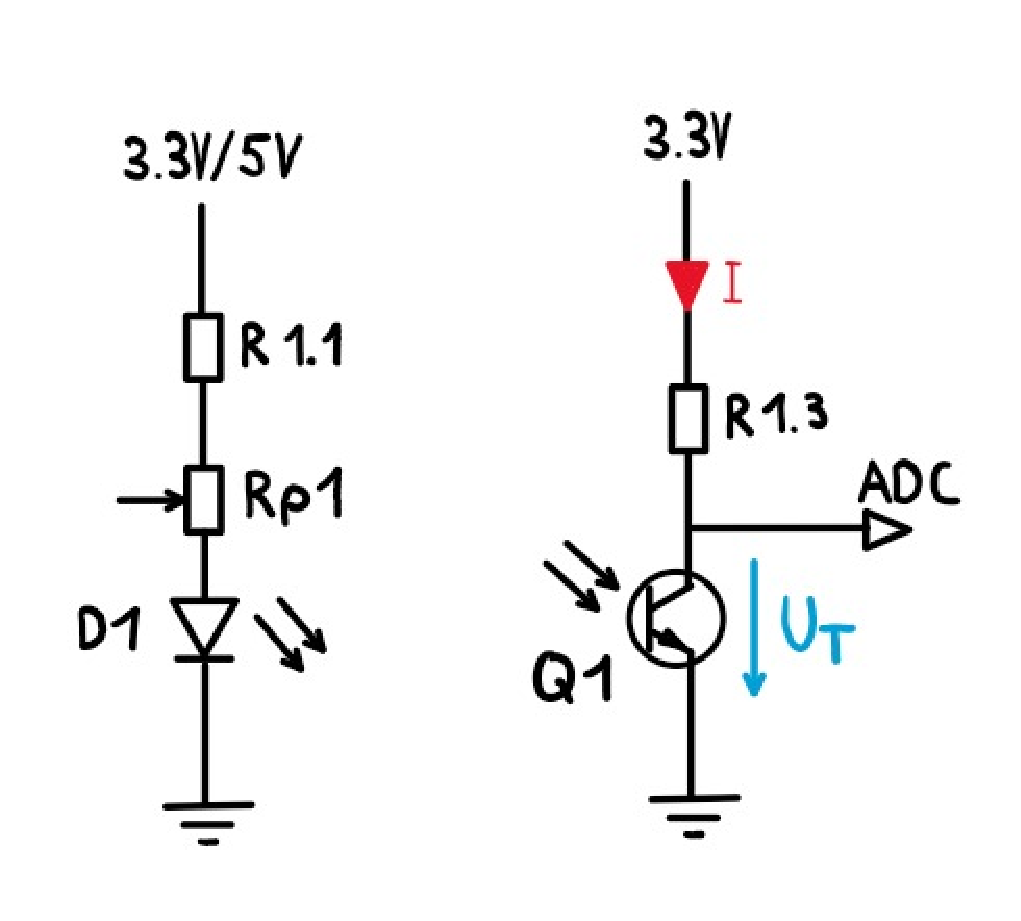
\includegraphics[width=0.5\textwidth]{fig_Strecke_Tracken/Schema_Messzelle_Liniensensor.pdf}
    \caption{Schema einer Messzelle}~\label{fig:Messzelle}
\end{figure}

Abbildung~\ref{fig:Messzelle} zeigt das Schema einer einzelnen Messzelle. Die Speisung von 5 V für 
den UV-Emitter ist notwendig, weil gemäss Datenblatt eine Spannung von 2.9 V bis 3.5 V abfällt. Daher reicht
eine Speisung von 3.3 V nicht aus. Ausserdem wurde als Sicherheitsmassnahme beim Messabgang über dem 
Fototransistor einen Platz für einen Widerstand eingebaut, damit bei allfälligen Stromspitzen der Strom 
limitiert werden könnte. Weil dies aber mit der verwendeten Auswertung nicht notwendig ist, wird ein
0 $\Omega$ Widerstand eingebaut. Die Potentiometer werden eingebaut, dass allfällige Bauteiltoleranzen
eliminiert werden können. Im Anhang~\ref{anhang:Liniensensor} wird dargestellt, wie die Werte der Komponenten $R_{1.1}$, $R_{p1}$ und $R_{1.3}$ 
dimensioniert werden.\\\\



% ===================================================================================


\subsubsection{Liniensensor als PCB}

Damit der Liniensensor möglichst praxisnah getestet 
werden kann, wird dieser als PCB mit dem CAD-Tool Kicad erstellt. Dabei werden die 
oben formulierten Anforderungen und Dimensionierungen eingehalten. In Abbildung~\ref{fig:Liniensensor_Top} 
ist die Draufsicht und in Abbildung~\ref{fig:Liniensensor_Bottom} die Untersicht dargestellt.

\begin{figure}[H]
    \centering
    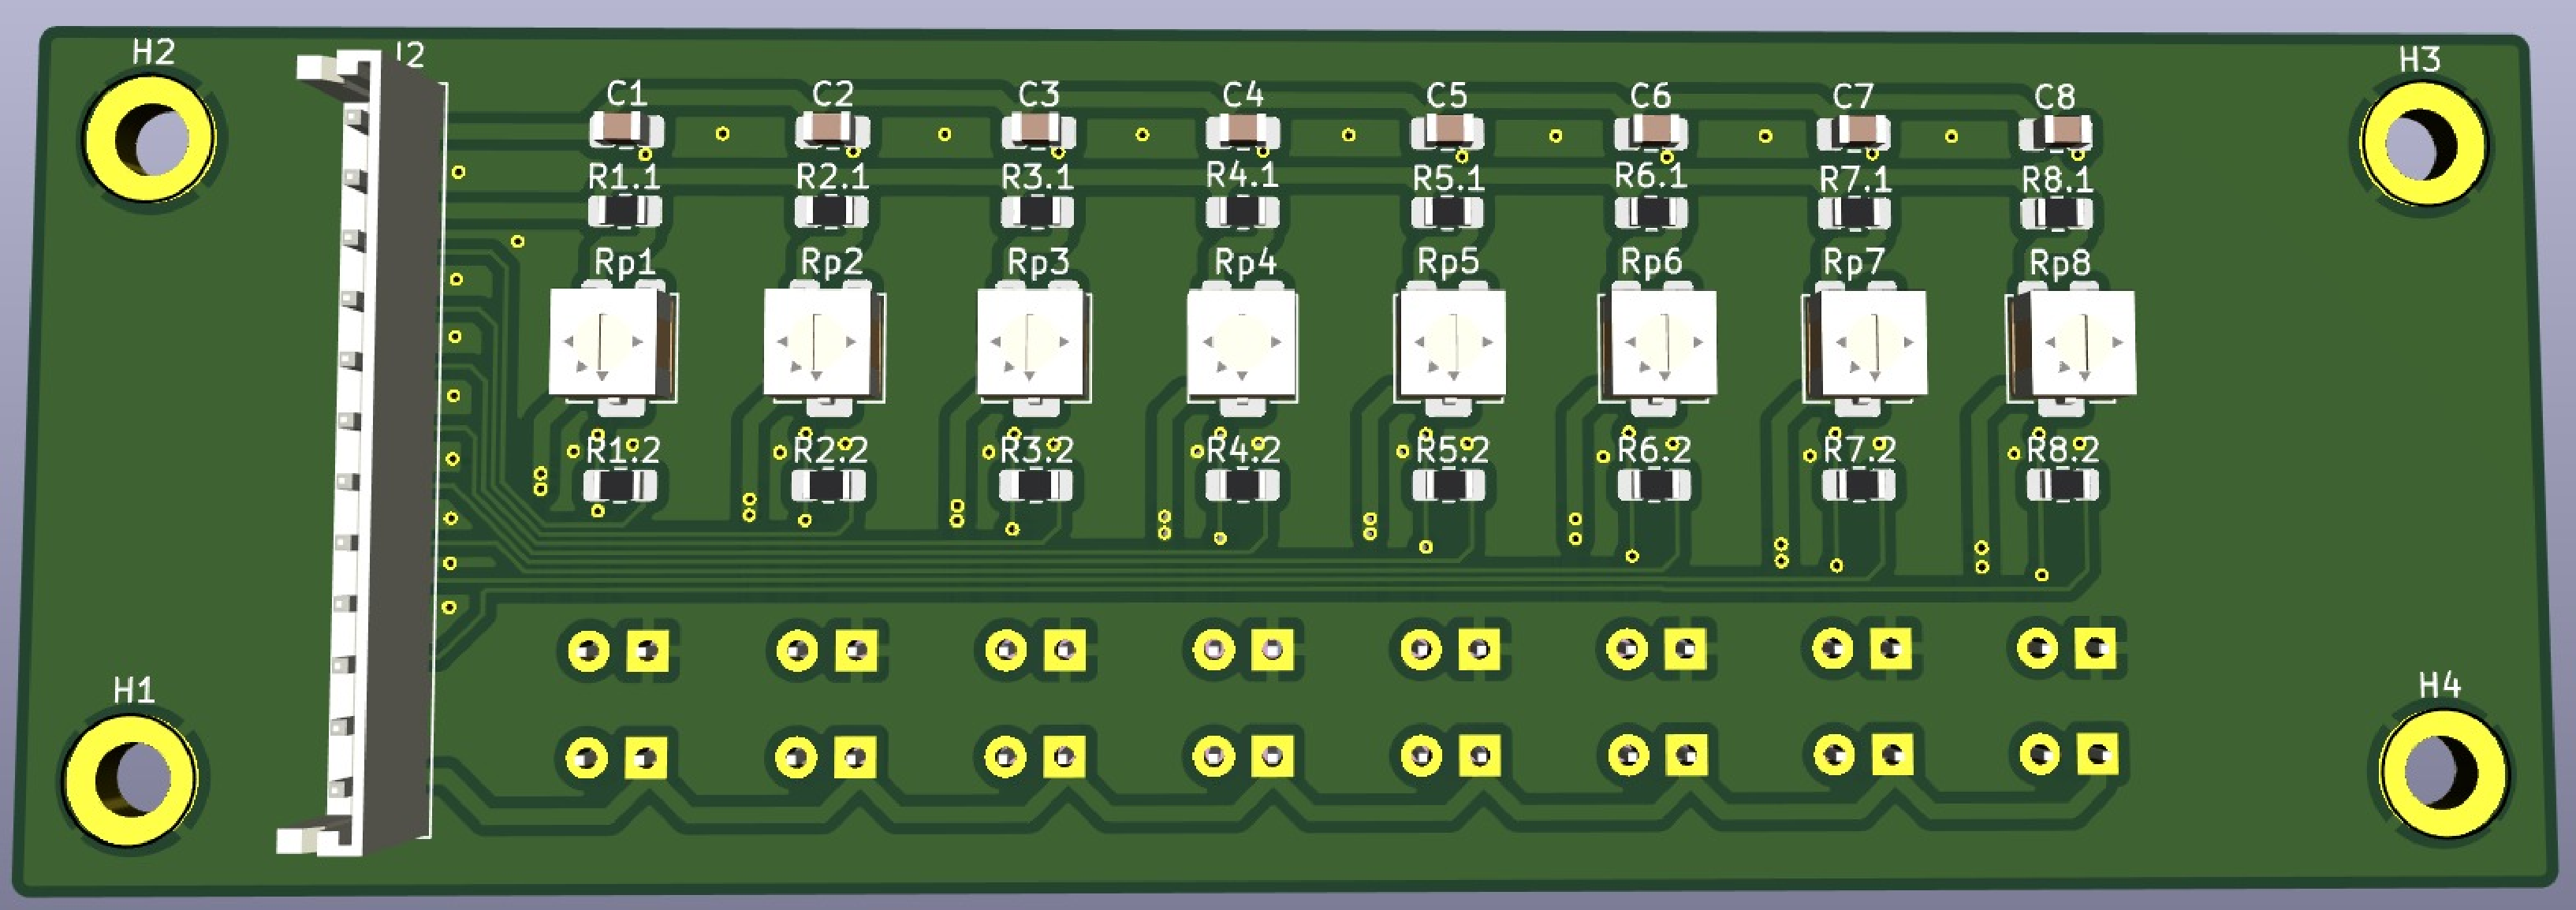
\includegraphics[width=0.75\textwidth]{fig_Strecke_Tracken/Liniensensor_Top.pdf}
    \caption{Liniensensor in Kicad von oben}~\label{fig:Liniensensor_Top}
\end{figure}

\begin{figure}[H]
    \centering
    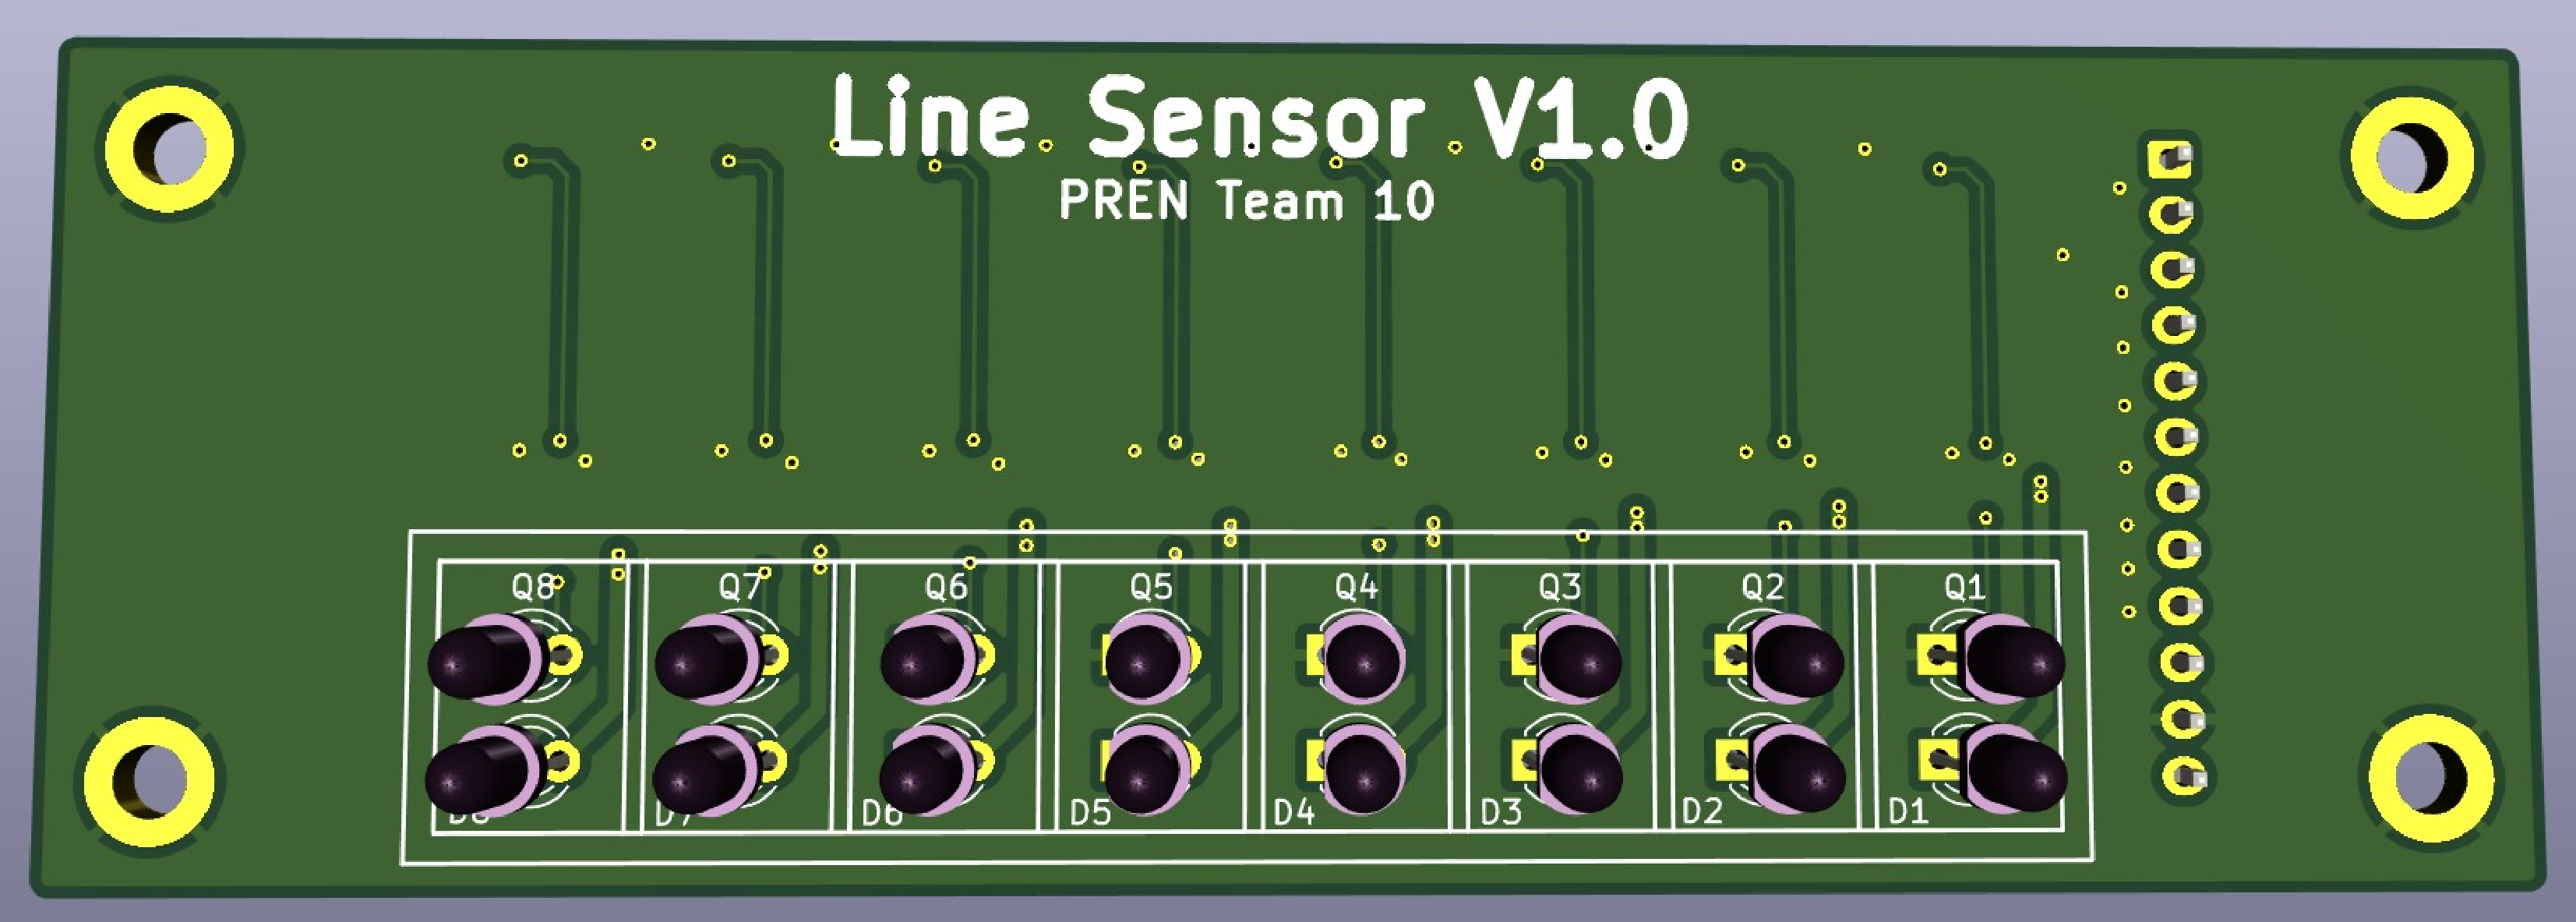
\includegraphics[width=0.75\textwidth]{fig_Strecke_Tracken/Liniensensor_Bottom.pdf}
    \caption{Liniensensor in Kicad von unten}~\label{fig:Liniensensor_Bottom}
\end{figure}




% ===================================================================================

\paragraph{Versuche}
Es wurde überprüft, welches Lichtspektrum am besten geeignet ist und die verschiedenen Ströme
durch den Fototransistor wurden getestet. Ausserdem wurde im UV-Spektrum die Spannungen über dem Fototransistor
gemessen. Mittels eines 
Arduino wurden für einen Test alle Eingänge ausgewertet und der Liniensensor validiert. 
Alle Messungen sind im Anhang~\ref{anhang:Liniensensor} dokumentiert.

% ===================================================================================
\paragraph{Entscheidung und Fazit}
Aufgrund der grossen Spannungsdifferenz zwischen Klebeband und Fliese/ Fuge, wurde eine mögliche
fluoreszierende Wirkung des Klebebandes im UV-Spektrum bestätigt. Durch die Messungen wurde das 
Konzept des Liniensensors überprüft und validiert. Das folgende Bild bestätigt, dass das Klebeband
von der Fliese deutlich unterschieden werden kann. Die Abbildung~\ref{fig:Auswertung_Strecke_Beispiel} zeigt
die Spannungsauswertung mittels ADCs. Diese Auswertung wurde mit einem Arduino gemacht. Die hohen 
Werte stellen die Fliese dar und die tiefen Werte das Klebeband.

\begin{figure}[H]
    \centering
    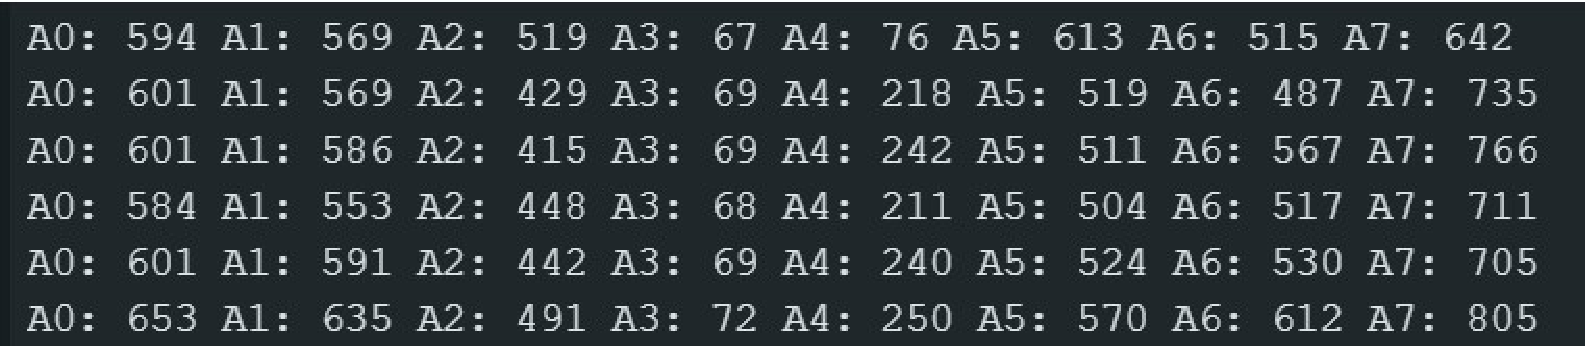
\includegraphics[width=0.75\textwidth]{fig_Strecke_Tracken/Auswertung_Strecke.pdf}
    \caption{Die tiefen Werte stellen das Klebeband dar und die hohen die Fliesen}~\label{fig:Auswertung_Strecke_Beispiel}
\end{figure}

Auf der Abbildung ist ersichtlich, dass sich A3 direkt überhalb dem Klebeband befindet. Die Pins A2 und A4 sind 
teilweise auch über dem Klebeband. Der Wert ist allerdings grösser, weil nur ein Teil des Klebebandes direkt darunter
liegt.\\
Anfangs wurde der Unterschied von Klebeband zu Fugen als eine Schwierigkeit betrachtet. Der Lininensensor ist fähig, 
Fugen von Klebeband zu unterscheiden. Dies ist im Anhang~\ref{anhang:Liniensensor} genauer dokumentiert.\\
Aufgrund der eindeutigen, im Anhang geschilderten  Messwerten, wird dieser Liniensensor verwendet.


\end{document}
